%% !TeX root = main.tex

\chapter{CORDIC}
\glsresetall
\label{chapter:cordic}

\section{Overview}
\label{subsec:CORDIC_Overview}

%\note{Is this the right place for this? I think it is fine. Just keep the focus on number representation. Do not do anything about pipelining, unrolling, memory partitioning, etc. That will be covered in the DFT chapter (next). Need to integrate the basic ideas of number representation (currently its own separate chapter) into this one. Also need to talk about some of the optimization tricks. E.g., the if/else to selection operator optimization. Can look through students old reports to see other common tricks.}

CORDIC (Coordinate Rotation DIgital Computer) is an efficient technique to calculate trigonometric, hyperbolic, and other mathematical functions. It is a digit-by-digit algorithm that produces one output digit per iteration. This allows us to tune the accuracy of the algorithm to the application requirements; additional iterations produce a more precise output result. Accuracy is another common design evaluation metric alongside performance and resource usage. CORDIC performs simple computations using only addition, subtraction, bit shifting, and table lookups, which are efficient to implement in FPGAs and more generally in hardware. 

\begin{aside}
The CORDIC method was developed by Jack Volder in the 1950's as a digital solution to replace an analog resolver for real-time navigation on a B-58 bomber. A resolver measures degrees of rotation. At that time hardware implementations of multiply operations were prohibitively expensive and CPUs had very limited amount of state. Thus the algorithm needed to have low complexity and use simple operations.  Over the years, it has been used in math co-processors \cite{duprat1993cordic}, linear systems \cite{ahmed1982highly}, radar signal processing \cite{andraka1996building}, Fourier transforms \cite{despain1974fourier}, and many other digital signal processing algorithms. It is now commonly used in FPGA designs. \VHLS uses a CORDIC core for calculating trigonometric functions and it is a common element of modern FPGA IP core libraries.
\end{aside}

%\note{Talk about what HLS optimizations this chapter will focus on (number representation) and optimization of precision vs area and performance. 

The goal of this chapter is to demonstrate how to create an optimized CORDIC core using high-level synthesis. We are gradually increasing the complexity of the types of hardware cores that we are developing as we progress through the book. The CORDIC method is an iterative algorithm; thus most of the computation is performed within a single \lstinline|for| loop. The code itself is not all that complex. However, understanding the code such that we can create an optimal hardware implementation requires deep insight. And a good HLS designer must always understand the computation if they wish to create the optimal design. Thus, we spend the early part of this chapter giving the mathematical and computational background of the CORDIC method.  

The major HLS optimization that we wish to highlight in this chapter is choosing the correct number representation for the variables. As we discuss later in the chapter, the designer must carefully tradeoff between the accuracy of the results, the performance, and resource utilization of the design. Number representation is one big factor in this tradeoff -- ``larger'' numbers (i.e., those with more bits) generally provide more precision at the cost of increased resource usage (more FFs and logic blocks) and reduced performance. We provide a background on number representation and arbitrary data types in Chapter \ref{sec:arbitrary_precision}. 

%This chapter is coupled with the project described in Chapter \ref{chapter:phase_detector} that allows more in-depth experimentation with the tradeoffs between precision (accuracy of the computation), resource usage, and performance. The aim of this chapter is to provide enough insight so that one can perform the exercises from that project, i.e., this chapter and that project are meant to complement each other. The goal of the project is to build a phase detector which uses a CORDIC and a complex matched filter which we have conveniently covered in this and the previous chapter. 

\section{Background}
\label{subsec:CORDIC_Basics}

The core idea behind the CORDIC is to efficiently perform a set of vector rotations in a two-dimensional plane. By overlaying these rotations with some simple control decisions, we can perform a variety of fundamental operations, e.g., trigonometric, hyperbolic, and logarithmic functions, real and complex multiplication, and matrix decompositions and factorizations.  CORDIC has been used in a wide range of applications including signal processing, robotics, communications, and many scientific computations. CORDIC is commonly used in FPGA design since it has a small resource usage. 

In the following, we walk through the process of how a CORDIC performs the sine and cosine of a given an input angle $\theta$. This is done using a series of vector rotations using only simple operations which are very efficient to implement in hardware. At the high level, the algorithm works using a series of rotations with the goal of reaching the target input angle $\theta$. The key innovation that makes this efficient is that the rotations can be done in a manner that requires minimal computation. In particular, we perform the rotations using multiplications by constant powers of two. This translates to simply moving bits around in hardware which is extremely efficient as it does not require any sort of logic.  

\begin{figure}
\centering
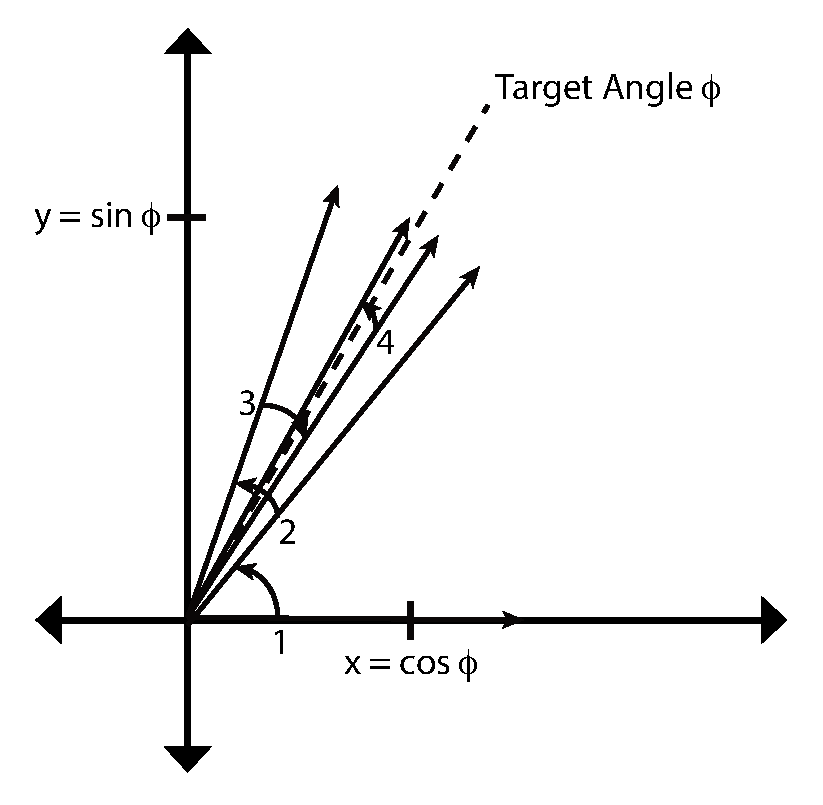
\includegraphics[width=.5\textwidth]{images/cordic_overview}
\caption{ Using the CORDIC to calculate the functions $\sin \phi$ and $\cos \phi$. Here, the CORDIC starts at the x-axis with a corresponding $0^\circ$ angle. It then performs four iterative positive/negative rotations in increasingly smaller rotation angle with the ultimate goal of reaching the target angle $\phi$. Once we finish our rotations we are close to the target angle. We take the corresponding $x$ and $y$ values of the final vector which correspond to  $\cos \phi$ and $\sin \phi$ (respectively) assuming the length of the vector is $1$. The key to the CORDIC is doing all of this in a computationally efficient manner. }
\label{fig:cordic_overview}
\end{figure}

Figure \ref{fig:cordic_overview} provides a high level overview of the CORDIC procedure for calculating $\cos \phi$ and $\sin \phi$. In this case, we start our initial rotating vector on the x-axis, i.e, at a $0^\circ$ angle. Then, we perform an iterative series of rotations; in this example we only perform four rotations, but generally this is on the order of 40 rotations. Each of the subsequent rotation uses an increasingly smaller angle, which means that every iteration adds a bit more precision to the output value. At each iteration, we decide between doing a positive or negative rotation by that smaller angle. The angle values that we rotate are fixed a priori; thus, we can easily store their values in a small memory and keep a running sum of the cumulative angle that we have rotated so far. If this cumulative angle is larger than our target angle $\phi$, then we perform a negative rotation. If it is smaller, then the rotation is positive. Once we have completed a sufficient number of rotations, we can determine the $\cos \phi$ and $\sin \phi$ by directly reading the $x$ and $y$ values from the final rotated vector. If our final vector has a magnitude of $1$, then $x = \cos \phi$ and $y = \sin \phi$.


We start with some terminology. The goal is to refresh your memory about some basic trigonometric and vector concepts. Feel free to skim this if it is familiar. But keep in mind that one of the most important aspects of creating an efficient hardware design is to truly understand the application; only then can the designer effectively utilize the optimization directives and perform code refactoring which is required to get the most efficient designs. 

The fundamental goal of the CORDIC algorithm is to perform a series of rotations in an efficient manner. Let us start by thinking about how to generally perform a rotation. In two dimensions, the rotation matrix is:
\begin{equation}
R(\theta) = \begin{bmatrix}
\cos \theta & -\sin \theta \\
\sin \theta & \cos \theta \\
\end{bmatrix}
\label{eq:rotation_matrix}
\end{equation}
The CORDIC uses an iterative algorithm that rotates a vector $v$ to some target of angle which depends on the function that the CORDIC is performing. One rotation is a matrix vector multiplications in the form of $v_{i} = R_{i} \cdot v_{i-1}$. Thus in each iteration of the CORDIC we perform the following operations to perform one rotation which is the matrix vector multiply:
\begin{equation}
\begin{bmatrix}
\cos \theta & -\sin \theta \\
\sin \theta & \cos \theta \\
\end{bmatrix}\begin{bmatrix}
x_{i-1} \\
y_{i-1} \\
\end{bmatrix}
= \begin{bmatrix}
x_i \\
y_i \\
\end{bmatrix} 
\end{equation}
Writing out the linear equations, the coordinates of the newly rotated vector are: 
\begin{equation}
x_i = x_{i-1}  \cos \theta - y_{i-1}  \sin \theta\
\end{equation} and 
\begin{equation}
y_i = x_{i-1} \sin \theta + y_{i-1} \cos \theta\
\end{equation}
This is precisely the operation that we need to simplify. We want to perform these rotations without having to perform any multiplications.

Consider first a $90^\circ$ rotation. In this case the rotation matrix is:
\begin{equation}
R(90^\circ) = \begin{bmatrix}
\cos 90^\circ & -\sin 90^\circ \\
\sin 90^\circ & \cos 90^\circ \\
\end{bmatrix} = \begin{bmatrix}
0 & -1 \\
1 & 0 \\
\end{bmatrix} 
\end{equation} and thus we only have to perform the operations:
%\begin{equation}
\begin{align}
x_i &= x_{i-1}  \cos 90^\circ - y_{i-1} \sin 90^\circ \nonumber \\
& = x_{i-1} \cdot 0 - y_{i-1} \cdot 1 \nonumber \\
& = -y_{i-1}\
\end{align}
%\end{equation} 
and 
\begin{align}
y_i &= x_{i-1} \sin  90^\circ + y_{i-1} \cos 90^\circ \nonumber \\
& = x_{i-1} \cdot 1 + y_{i-1} \cdot 0 \nonumber \\
&=  x_{i-1}\
\end{align}
Putting this altogether we get
\begin{equation}
\begin{bmatrix}
0 & -1 \\
1 & 0 \\
\end{bmatrix}\begin{bmatrix}
x \\
y \\
\end{bmatrix}
= \begin{bmatrix}
-y \\
x \\
\end{bmatrix} 
\end{equation}
You can see that this is requires a very minimal amount of calculation; the rotated vector simply negates the $y$ value, and then swaps the $x$ and $y$ values. A two's complement negation requires the hardware equivalent to an adder. Thus, we have achieved our goal of performing a $90^\circ$ rotation efficiently.

\begin{exercise}
What if you wanted to rotation by $-90^\circ$? What is the rotation matrix $R(-90^\circ)$? What type of calculation is required for this rotation? How would one design the most efficient circuit that could perform a positive and negative rotation by $-90^\circ$, i.e., the direction of rotation is an input to the circuit?
\end{exercise}

While it is great that we can rotate by $\pm 90^\circ$, we also need to rotate by smaller angles if we wish to have any sort of good resolution in moving to the target angle. Perhaps the next natural angle that we might wish to rotate would be $\pm 45^\circ$. Using the rotation matrix from Equation \ref{eq:rotation_matrix}, we get
\begin{equation}
R(45^\circ) = \begin{bmatrix}
\cos 45^\circ & -\sin 45^\circ \\
\sin 45^\circ & \cos 45^\circ \\
\end{bmatrix} = \begin{bmatrix}
\sqrt 2/2 & -\sqrt 2/2 \\
\sqrt 2/2 & \sqrt 2/2 \\
\end{bmatrix}
\end{equation} Calculating out the computation for performing the rotation, we get
\begin{align}
x_i &= x_{i-1}  \cos 45^\circ - y_{i-1} \sin 45^\circ \nonumber \\
& = x_{i-1} \cdot \sqrt 2/2  - y_{i-1} \cdot \sqrt 2/2
\end{align} and 
\begin{align}
y_i &= x_{i-1} \sin  45^\circ + y_{i-1} \cos 45^\circ \nonumber \\
&= x_{i-1} \cdot \sqrt 2/2 + y_{i-1} \cdot \sqrt 2/2
\end{align} which when put back into matrix vector notation is
\begin{equation}
\begin{bmatrix}
\sqrt 2/2 & -\sqrt 2/2 \\
\sqrt 2/2 & \sqrt 2/2 \\
\end{bmatrix}
\begin{bmatrix}
x \\
y \\
\end{bmatrix}
= \begin{bmatrix}
\sqrt 2/2 x - \sqrt 2/2 y \\
\sqrt 2/2 x + \sqrt 2/2 y \\
\end{bmatrix} 
\end{equation}
This certainly is not as efficient of a computation as compared to rotating by $\pm 90^\circ$. The $\pm 90^\circ$ rotation was ideal because the multiplication were by very simple constants (in this case $0$, $1$, and $-1$). The key to the CORDIC is doing these rotations in an efficient manner, i.e., defining the rotation matrix in a way that their multiplication is trivial to compute. That is, we wish to be more like the previous $\pm 90^\circ$ and less like the much more difficult computation required for the $\pm 45^\circ$ rotation that we just described.

What if we ``forced'' the rotation matrix to be constants that were easy to multiply? For example, a multiplication by any power of two turns into a shift operation. If we set the constants in the rotation matrix to be powers of two, we could very easily perform rotations without multiplication. This is the key idea behind the CORDIC -- finding rotations that are very efficient to compute while minimizing any side effects. We will discuss these ``side effects'' in more detail, but there is an engineering decision that is being made here. In order to get efficient computation, we have to give up something; in this case we have to deal with the fact that the rotation also performs scaling, i.e., it changes the magnitude of the rotated vector  -- more on that later.

To further explore the idea of ``simple'' rotation matrices, consider the matrix 
\begin{equation}
R() = \begin{bmatrix}
1 & -1 \\
1 & 1 \\
\end{bmatrix} 
\end{equation} with the corresponding computation for the transformation
\begin{equation}
x_i = x_{i-1}  - y_{i-1}\
\end{equation} and 
\begin{equation}
y_i = x_{i-1}  + y_{i-1}\
\end{equation} with the matrix vector form of
\begin{equation}
\begin{bmatrix}
1 & -1 \\ 
1 & 1 \\
\end{bmatrix}
\begin{bmatrix}
x \\
y \\
\end{bmatrix}
= \begin{bmatrix}
x - y \\
x + y \\
\end{bmatrix} 
\end{equation}

This is certainly easy to compute and does not require any ``difficult'' multiplications. But what is the consequence of this operation? It turns out that this performs a rotation by $45^\circ$ which is perfect; we now have an efficient way to perform a $45^\circ$ rotation. But, this transform also scales the vector by a factor of  $\sqrt 2$.  The square root of the determinant of this matrix tells us how much the transformation scales the vector, i.e., how the length of the vector has changed. The determinant of this matrix here is $1 \cdot 1 -  (-1) \cdot 1 = 2$. Thus, this operation rotates by $45^\circ$ and scales by $\sqrt 2$. This is the tradeoff that the CORDIC makes; we can make the computation for the rotation easy to compute but it has the side effect that scales the length of the vector. This may or may not be a problem depending on the application. But for now, we put aside the scaling issue and focus on how to generalize the idea of performing rotations that are computationally efficient to perform.

Now we generalize the notion of performing efficient matrix rotations, i.e., performing rotations by only performing addition/subtraction and multiplication by a power of two (i.e., by shift operations). Consider again the rotation matrix 

\begin{equation}
R_{i}(\theta) = \begin{bmatrix} \cos(\theta_{i}) & -\sin(\theta_{i}) \\ \sin(\theta_{i}) & \cos(\theta_{i})\end{bmatrix}
\end{equation}
By using the following trigonometric identities,
\begin{equation}
\cos(\theta_{i}) =  {\frac{1}{\sqrt{1 + \tan^2(\theta_{i})}}}
%\sin(\gamma_{i}) & =  \frac{\tan(\gamma_{i})}{\sqrt{1 + \tan^2(\gamma_{i})}} \end{align}
\end{equation}
\begin{equation}
\sin(\theta_{i})  =  \frac{\tan(\theta_{i})}{\sqrt{1 + \tan^2(\theta_{i})}}
\end{equation}
we can rewrite the rotation matrix as
\begin{equation}
R_i = \frac{1}{\sqrt{1 + \tan^2(\theta_i)}} \begin{bmatrix} 1 & -\tan(\theta_i) \\ \tan(\theta_i) & 1 \end{bmatrix}
\end{equation}
If we restrict the values of $\tan(\theta_i)$ to be a multiplication by a factor of two, the rotation can be performed using shifts (for the multiplication) and additions. More specifically, we use let $\tan(\theta_i) = 2^{-i}$. The rotation then becomes 
\begin{equation}
v_i = K_i \begin{bmatrix} 1 & - 2^{-i} \\  2^{-i} & 1 \end{bmatrix} \begin{bmatrix} x_{i-1} \\ y_{i-1} \end{bmatrix}
\end{equation}
where
\begin{equation}
K_i = \frac{1}{\sqrt{1 + 2^{-2i}}}
\end{equation}

A few things to note here. The $2^{-i}$ is equivalent to a right shift by $i$ bits, i.e., a division by a power of two. This is essentially just a simple rewiring which does not require any sort of logical resources, i.e., it is essentially ``free'' to compute in hardware. This is a huge benefit, but it does not come without some drawbacks. First, we are limited to rotate by angles $\theta$ such that $\tan(\theta_i) = 2^{-i}$. We will show that this is not much of a problem. Second, we are only showing rotation in one direction; the CORDIC requires the ability to rotation by $\pm \theta$. This is simple to correct by adding in $\sigma$ which can have a value of $1$ or $-1$, which corresponds to performing a positive or negative rotation. We can have a different $\sigma_i$ at every iteration/rotation. Thus the rotation operation generalizes to
\begin{equation}
v_i = K_i \begin{bmatrix} 1 & -\sigma_i 2^{-i} \\ \sigma_i 2^{-i} & 1 \end{bmatrix} \begin{bmatrix} x_{i-1} \\ y_{i-1} \end{bmatrix}
\end{equation}
Finally, the rotation requires a multiplication by $K_i$.  $K_i$ is typically ignored in the iterative process and then adjusted for after the series of rotations is completed. The cumulative scaling factor is
\begin{equation}
K(n) = \prod_{i=0}^{n-1} K_i  = \prod_{i=0}^{n-1}\frac {1}{\sqrt{1 + 2^{-2i}}}
\end{equation} and  
\begin{equation}
K = \lim_{n \to \infty}K(n) \approx 0.6072529350088812561694
\end{equation}
The scaling factors for different iterations can be calculated in advance and stored in a table. If we always perform a fixed number of rotations, this is simply one constant. This correction could also be made in advance by scaling $v_0$ appropriately before performing the rotations. Sometimes it is ok to ignore this scaling, which results in a processing gain
\begin{equation}
A = \frac{1}{K} = \lim_{n \to \infty} \prod_{i=0}^{n-1} {\sqrt{1 + 2^{-2i}}}\approx 1.64676025812107
\label{eq:cordicgain}
\end{equation}

At each iteration, we need to know the angle $\theta_i$ of the rotation that was just performed. This is derived as $\theta_i = \arctan 2^{-i}$. We can precompute these values for each value of $i$ and store them in an on-chip memory and use them as a lookup table. Additionally, we have a control decision that determines whether the rotation is clockwise or counterclockwise, i.e., we must determine if $\sigma$ is $1$ or $-1$. This decision depends on the desired CORDIC mode. For example, for calculating $\cos \phi$ and $\sin \phi$, we keep a running sum of the cumulative angle that we have rotated so far. We compare this to the target angle $\phi$ and perform a positive rotation if our current angle is less than $\phi$ and a negative rotation is our current angle is greater than $\phi$. 

Table \ref{table:cordic} provides the statistics for the first seven iterations of a CORDIC. The first row is the ``zeroth'' rotation (i.e., when $i=0$), which is a $45^{\circ}$ rotation. It performs a scaling of the vector by a factor of $1.41421$. The second row is the does a rotation by $2^{-1} = 0.5$. This results in a rotation by $\theta = \arctan 2^{-1} = 26.565^{\circ}$. This rotation scales the vector by $1.11803$. The CORDIC gain is the overall scaling of the vector. In this case, it is the scaling factor of the first two rotations, i.e., $1.58114 = 1.41421 \cdot 1.11803$. This process continues by incrementing $i$ which results in smaller and smaller rotating angles and scaling factors. Note that the CORDIC gain starts to stabilize to $\approx 1.64676025812107$ as described in Equation \ref{eq:cordicgain}. Also, note as the angles get smaller, they have less effect on the most significant digits. 

\begin{exercise}
Describe the effect if the $i$th iteration on the precision of the results? That is, what bits does it change? How does more iterations change the precision of the final result, i.e., how do the values of $\sin \phi$ and $\cos \phi$ change as the CORDIC performs more iterations?
\end{exercise}



\begin{table}[htbp]
\caption{The rotating angle, scaling factor, and CORDIC gain for the first seven iterations of a CORDIC. Note that the angle decreases by approximately half each time. The scaling factor indicates how much the length the the vector increases during that rotation. The CORDIC gain is the overall increase in the length of the vector which is the product of all of the scaling factors for the current and previous rotations.}
\begin{center}
\begin{tabular}{|c|c|c|c|c|c|}
\hline
i & $2^{-i}$ 	& Rotating Angle  	& Scaling Factor 	& CORDIC Gain 	\\ \hline \hline
0 & 1.0 		& $45.000^{\circ}$	& 1.41421			& 1.41421		\\ \hline
1 & 0.5 		& $26.565^{\circ}$	& 1.11803			& 1.58114		\\ \hline
2 & 0.25 		& $14.036^{\circ}$	& 1.03078			& 1.62980		\\ \hline
3 & 0.125 		& $7.125^{\circ}$	& 1.00778			& 1.64248		\\ \hline
4 & 0.0625 	& $3.576^{\circ}$	& 1.00195			& 1.64569		\\ \hline
5 & 0.03125 	& $1.790^{\circ}$	& 1.00049			& 1.64649		\\ \hline
6 & 0.015625 	& $0.895^{\circ}$	& 1.00012			& 1.64669		\\ \hline
\end{tabular}
\end{center}
\label{table:cordic}
\end{table}%

\section{Calculating Sine and Cosine}

Now we describe more precisely our running example of using a CORDIC to calculate the sine and cosine of some given angle $\phi$. In order to do this, we start with a vector on the positive $x$-axis (i.e., with an initial angle of $0^{\circ}$) and perform a series of rotations until we are approximately at the given angle $\phi$. Then we can simply read the $x$ and $y$ values of the resulting rotated vector to get the values $\cos \phi$ and $\sin \phi$, respectively. This assumes that the amplitude of the final vector is equal to $1$, which as you will see is not too difficult to achieve.

\begin{figure}
\centering
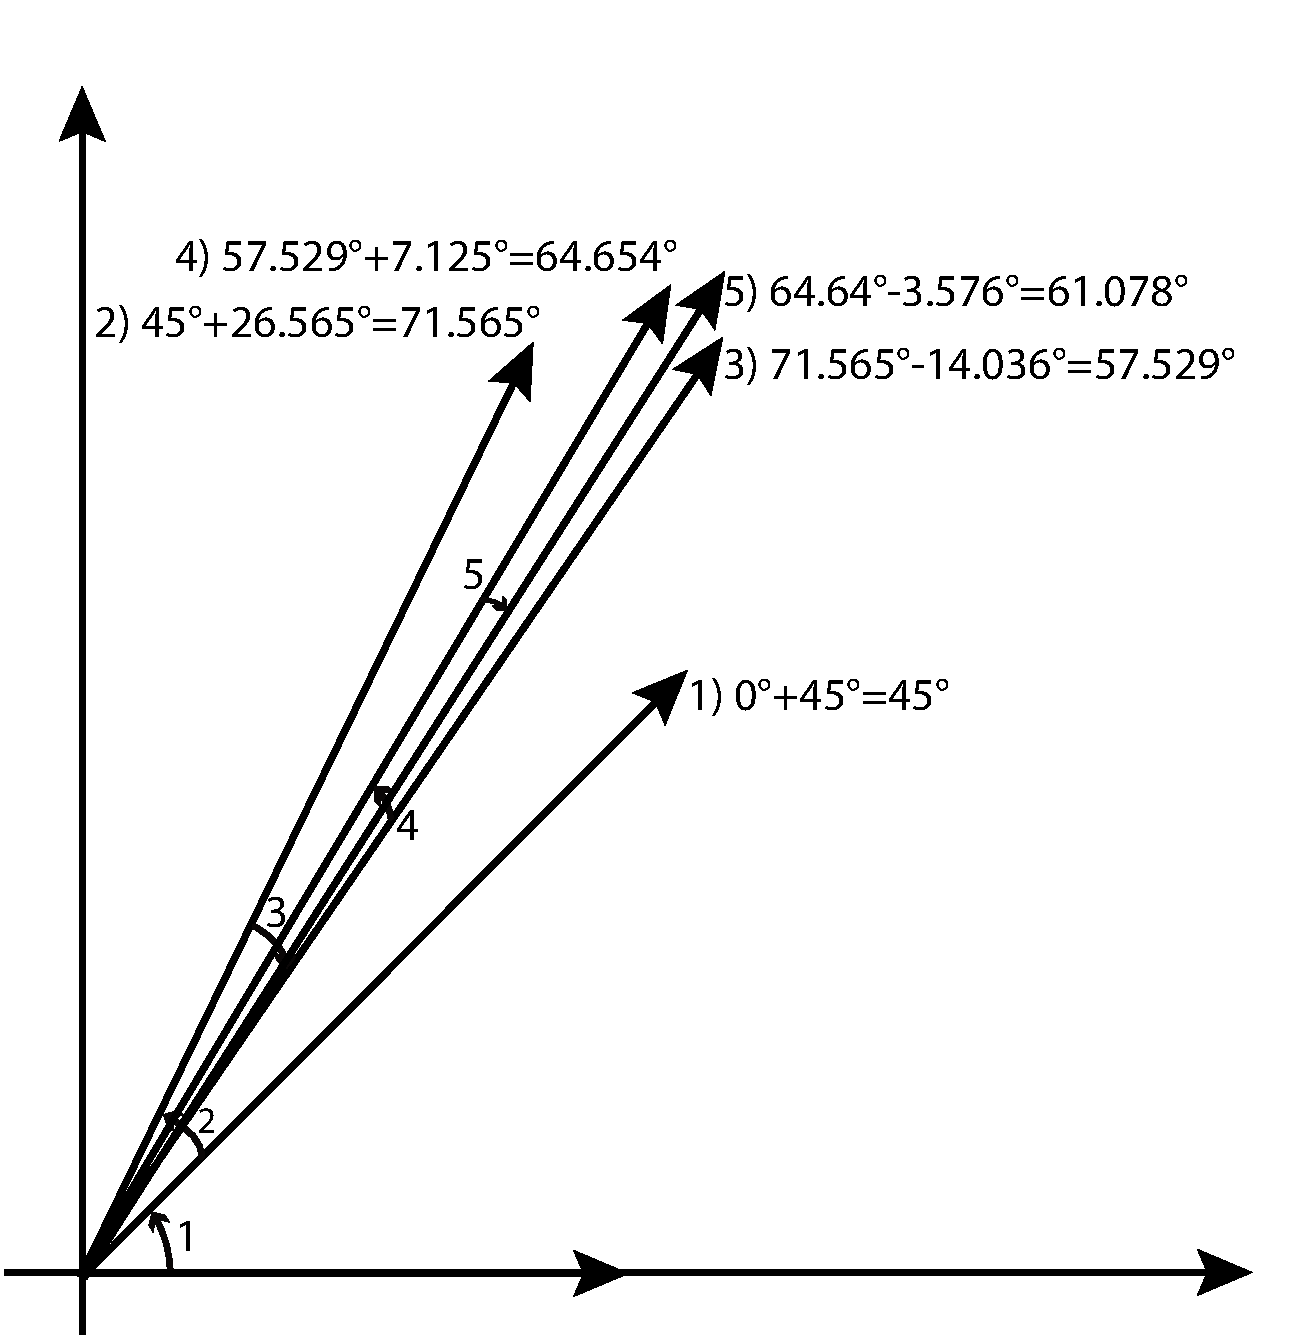
\includegraphics[width=.5\textwidth]{images/sin_cos_cordic}
\caption{Calculating $\cos 60^{\circ}$ and $\sin 60^{\circ}$ using the CORDIC algorithm. Five rotations are performed using incrementally larger $i$ values (0,1,2,3,4). The result is a vector with an angle of $61.078^{\circ}$. The corresponding $x$ and $y$ values of that vector give the approximate desired cosine and sine values. }
\label{fig:cordic_rotations}
\end{figure}

Let us illustrate this with an example: calculating $ \cos 60^{\circ}$ and $\sin 60^{\circ}$, i.e., $\phi = 60^{\circ}$. This process is depicted graphically in Figure \ref{fig:cordic_rotations}. Here we perform five rotations in order to give a final vector with an angle approximately equal to $60^{\circ}$. Our initial vector has a $0^{\circ}$ angle, i.e., it starts on the positive $x$-axis. The first rotation corresponds to $i=0$ which has a $45^{\circ}$ angle (see Table \ref{table:cordic}). Since we want to get to $60^{\circ}$, we rotate in the positive direction. The resulting rotated vector has a $45^{\circ}$ angle; also note that its amplitude is scaled by approximately 1.414. Now, we move on to $i=1$. As we wish to get to a $60^{\circ}$ angle, we rotate again in the positive direction. This rotation results in a vector that has an angle of $45^{\circ} + 26.565^{\circ} = 71.565^{\circ}$ and is scaled by a factor of 1.118; the total scaling resulting from the two rotations is $1.414 \times 1.118 = 1.581$. This is the CORDIC gain. Moving on to $i=2$, we now determine that our current angle is larger than the $60^{\circ}$ target, so we rotate by a negative angle resulting in a vector with a $57.529^{\circ}$ angle and scaled by a factor of $1.630$. This process continues by rotating the vector with incrementally larger $i$ values, resulting in smaller and smaller rotations that will eventually (approximately) reach the desired angle.  Also, note that the CORDIC gain begins to stabilize as the number of rotation increases.

After we perform a sufficient number of rotations, which is a function of the desired accuracy, we get a vector with an angle close to the desired input angle. The $x$ and $y$ values of that vector correspond to approximately $A_R \cos 60^{\circ}$ and $A_R \sin 60^{\circ}$, which is exactly what we want if $A_R = 1$. Since we typically know a priori the number of rotations that we will perform, we can insure that $A_R = 1$ by setting the magnitude of the initial vector to the reciprocal of the CORDIC gain. In the case of our example, assuming that we perform five rotations as shown in Figure \ref{fig:cordic_rotations}, this value is $1.64649^{-1} = 0.60735$ (the reciprocal of the CORDIC gain when $i=5$; see Table \ref{table:cordic}). We can easily set the amplitude of the initial vector by starting at a vector $(0.60735, 0)$. 

\begin{exercise}
How would the answer change if we performed one more rotation? How about two (three, four, etc.) more rotations? What is the accuracy (e.g., compared to MATLAB implementation) as we perform more rotations? How many rotations do you think is sufficient in the general case?
\end{exercise}


\begin{exercise}
Is it possible to get worse accuracy by performing more rotations? Provide an example when this would occur.
\end{exercise}

\begin{figure}
\lstinputlisting{examples/cordic.cpp}
\caption{CORDIC code implementing the sine and cosine of a given angle.}
\label{fig:cordic_code}
\end{figure}

Figure \ref{fig:cordic_code} provides code that implements sine and cosine calculation using the CORDIC algorithm. It takes as input a target angle, and outputs the sine and cosine values corresponding to that angle. The code uses an array \lstinline{cordic_phase} as a lookup table that holds the angle of rotation for each iteration. This corresponds to the values in the ``Rotating Angle'' column in Table \ref{table:cordic}. We assume that the \lstinline{cordic.h} file defines the different data types (i.e., \lstinline{COS_SIN_TYPE} and \lstinline{THETA_TYPE}) and sets \lstinline{NUM_ITERATIONS} to some constant value. The data types can be changed to different fixed or floating point types, and \lstinline{NUM_ITERATIONS} set depending on our desired accuracy, area, and throughput. 

This code is close to a ``software'' version. It can be optimized in many ways to increase its performance and reduce its area. We will discuss how to optimize this code later in the chapter.

\section{Cartesian to Polar Conversion}

With some modifications, the CORDIC can perform other functions. For example, it can convert between Cartesian and polar representations; we describe that in more detail in this section. The CORDIC can also do many other functions, which we will leave as an exercise to the reader. 

A two-dimensional vector $v$ can be represented using a Cartesian coordinate system $(x, y)$ or in the polar coordinate system $(r, \theta)$ where  $r$ is the radial coordinate (length of the vector) and $\theta$ is the angular coordinate. Both of these coordinate systems have their benefits and drawbacks. For example, if we want to do a rotation, then it is easier to think about the polar form while a linear transform is more easily described using the Cartesian system. 

\begin{figure}
\centering
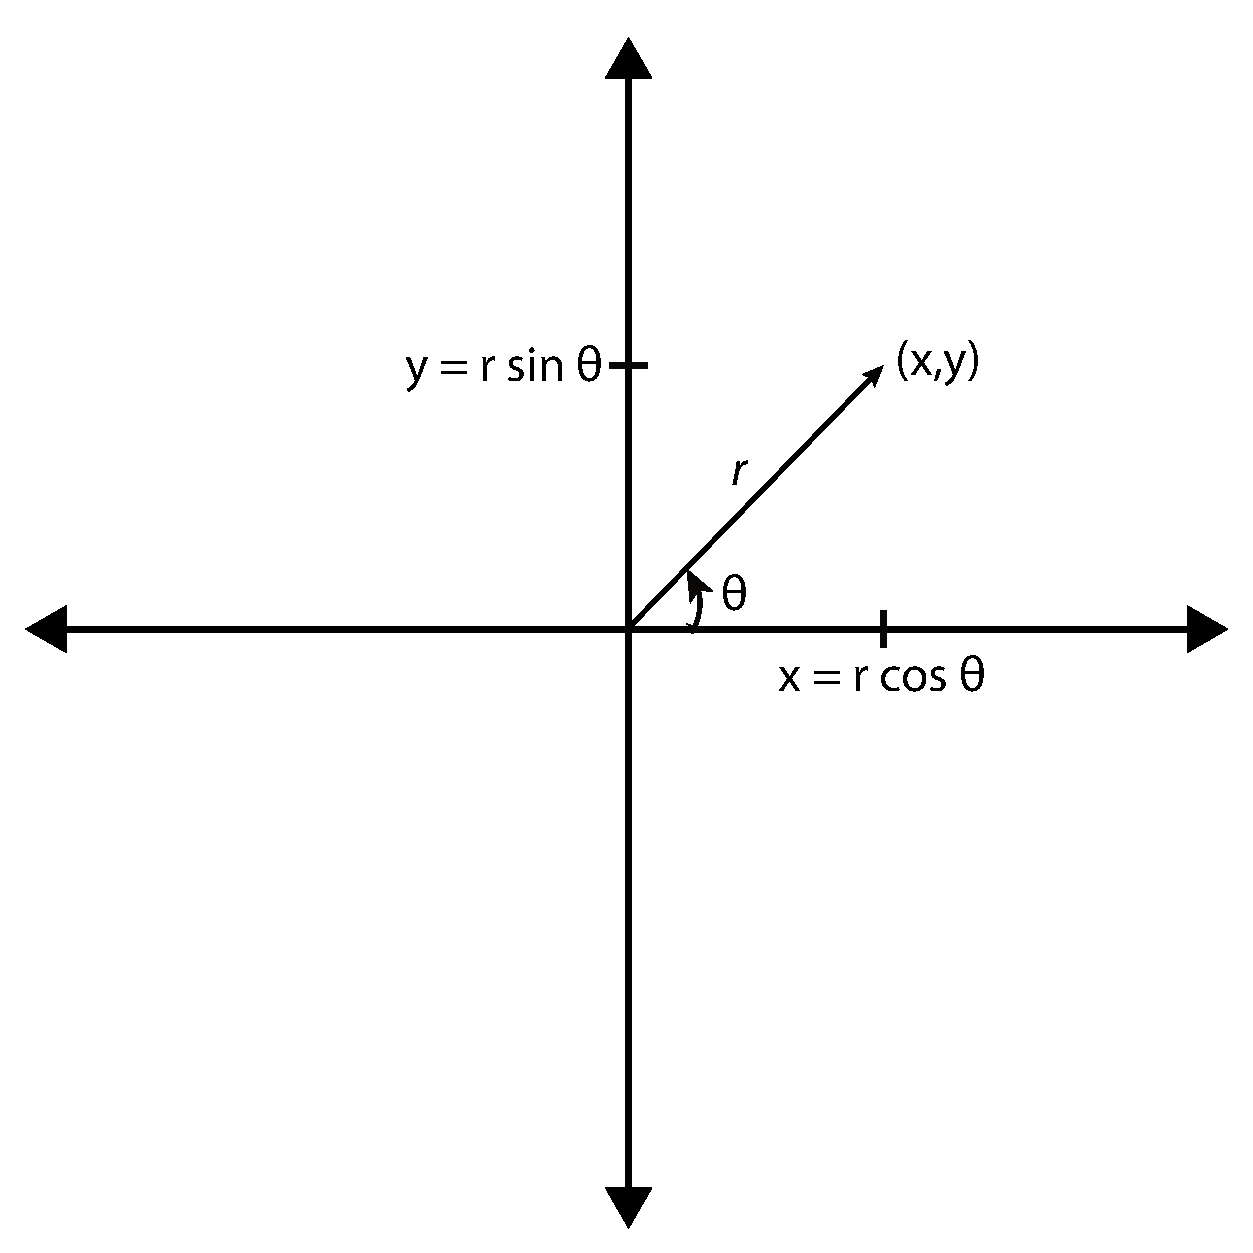
\includegraphics[width=.55\textwidth]{images/rotation}
\caption{ The figure shows a two-dimensional plane and a vector represented in both the Cartesian form $(x,y)$ and the polar form $(r, \theta)$ and provides the relationship between those two coordinate systems.  }
\label{fig:cordic_polar}
\end{figure}

The relationship between these coordinates is shown in the following equations:

\begin{equation}
x = r \cos \theta
\end{equation}

\begin{equation}
y = r \sin \theta
\end{equation}

\begin{equation}
r =\sqrt{x^2 + y^2}
\end{equation}

\begin{equation}
\theta = \operatorname{atan2}(y, x)
\end{equation}
where atan2 is a common variation on the arctangent function defined as
\begin{equation}
\operatorname{atan2}(y, x) =
\begin{cases}
\arctan(\frac{y}{x}) & \mbox{if } x > 0\\
\arctan(\frac{y}{x}) + \pi & \mbox{if } x < 0 \mbox{ and } y \ge 0\\
\arctan(\frac{y}{x}) - \pi & \mbox{if } x < 0 \mbox{ and } y < 0\\
\frac{\pi}{2} & \mbox{if } x = 0 \mbox{ and } y > 0\\
-\frac{\pi}{2} & \mbox{if } x = 0 \mbox{ and } y < 0\\
\text{undefined} & \mbox{if } x = 0 \mbox{ and } y = 0
\end{cases}
\end{equation}

This provides a way to translate between the two coordinate systems. However, these operations are not easy to implement in hardware. For example, sine, cosine, square root, and arctan are not simple operations and they require significant amount of resources. But we can use the CORDIC to perform these operations using a series of simple iterative rotation operations. 

Given a number in Cartesian form $(x,y)$, we can calculates its radial and amplitude coordinate (i.e., convert it to polar form) using the CORDIC. To do this, we rotate the given Cartesian number to $0^{\circ}$. Once this rotation is complete, the amplitude is the $x$ value of the final rotated vector. To determine the radial coordinate, we simply keep track of the cumulative angle of the rotations that the CORDIC performs. The angles of the rotating vector (for $i = 0,1,2,3, \dots$) are known and can be stored in a lookup table as done for calculating sine/cosine. Therefore, we simply need to keep track of the total rotation angle by performing an addition or subtraction of these angles, which depends on the direction of rotation.

The algorithm is similar to that of calculating the sine and cosine of a given angle. We perform a set of rotations with increasing values of $i$ such that the final vector resides on (close to) the positive $x$-axis (i.e., an angle of $0^{\circ}$). This can be done using positive or negative rotations  which is predicated on the $y$ value of the vector whose amplitude and phase we wish to determine. 

The first step of the algorithm performs a rotation to get the initial vector into either Quadrant I or IV. This rotates the vector by $\pm 90^{\circ}$ depending on the sign of the $y$ value of the initial vector. If the $y$ value is positive, we know that we are in either Quadrant I or II. A rotation by $-90^{\circ}$ will put us into Quadrant IV or I, respectively. Once we are in either of those quadrants, we can guarantee that we will be able to asymptotically approach the target $0^{\circ}$ angle. If we are in Quadrant III or IV, the $y$ value of the initial vector will be negative. And a rotation by $90^{\circ}$ will put us into Quadrant IV or I, respectively. Recall that a $\pm 90^{\circ}$ rotation is done by negating either the $x$ or $y$ values of the vector and then swapping those values. The concept of these $\pm 90^{\circ}$ is shown in Figure \ref{fig:rotate90}.

\begin{figure}
\centering
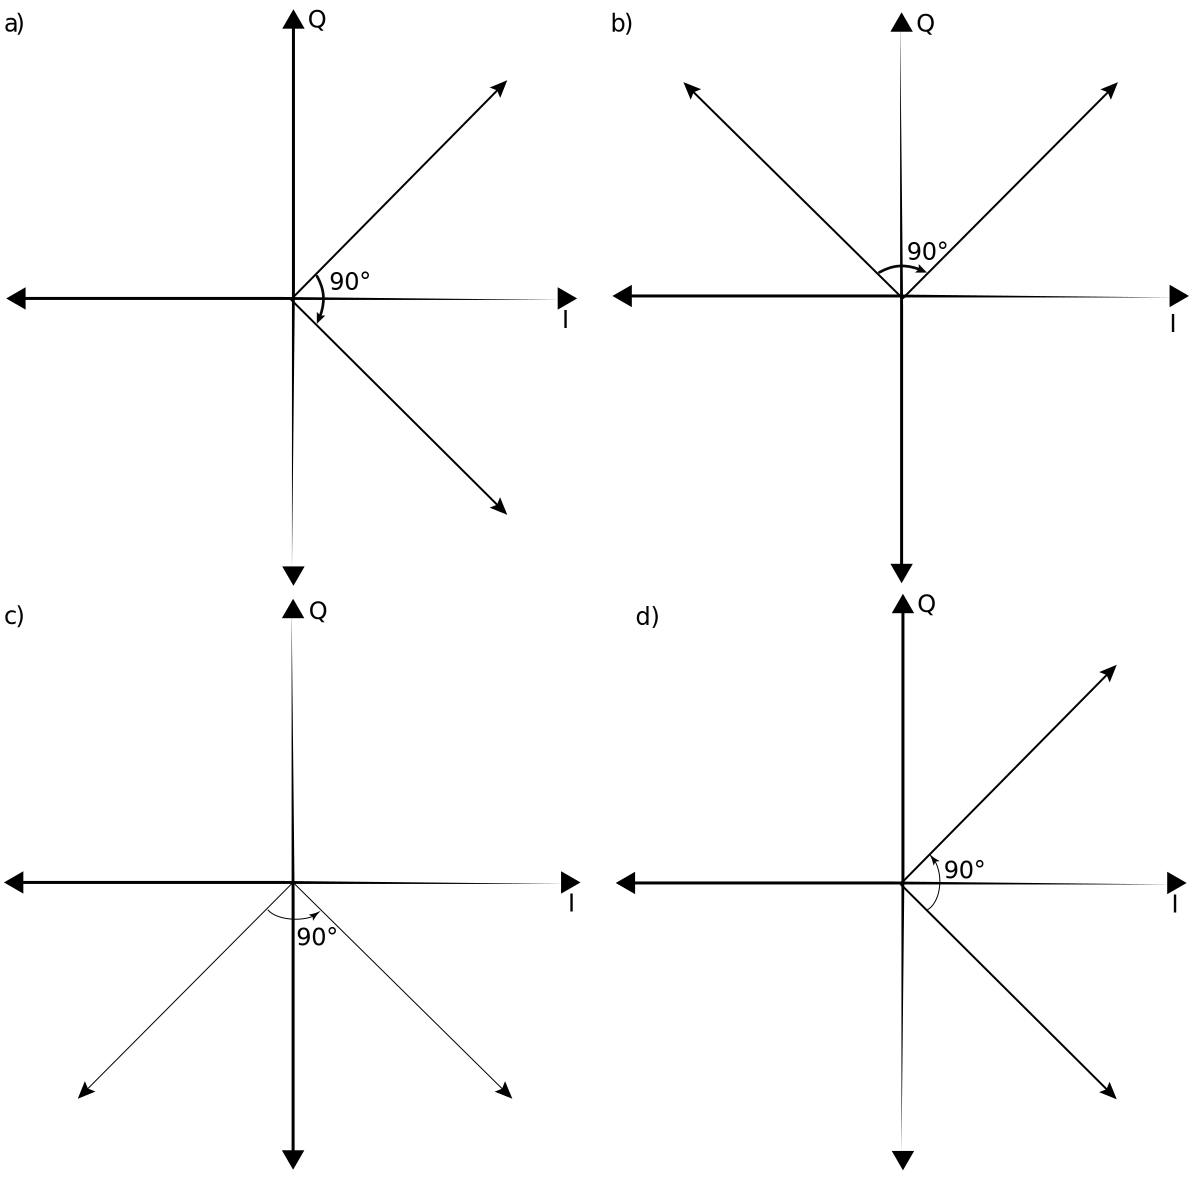
\includegraphics[width=\textwidth]{images/cordic_magnitude_angle}
\caption{The first step in performing a Cartesian to polar conversion is to perform a rotation by $\pm 90^{\circ}$ in order to get the initial vector into either Quadrant I or IV. Once it is in either of these two quadrants, subsequent rotations will allow the vector to reach a final angle of $0^{\circ}$. At this point, the radial value of the initial vector is the $x$ value of the final rotated vector and the phase of the initial vector is the summation of all the angles that the CORDIC performed. Parts a) and b) show an example with the initial $y$ value is positive, which means that the vector resides in either Quadrant I or II. Rotating by $-90^{\circ}$ puts them into the appropriate quadrant. Parts c) and d) show a similar situation when the $y$ value of the initial vector is negative. Here we wish to rotate by $90^{\circ}$ to get the vector into Quadrant I or IV. }
\label{fig:rotate90}
\end{figure}

There is an issue with the final radial value of the rotated vector; its magnitude is not the same as the initial magnitude before the rotations; it is scaled by the CORDIC gain. Or course, one could calculate the precise radial value of the vector by multiplying by the reciprocal of the appropriate CORDIC gain (approximately $1/1.647 = 0.607$)\footnote{Recall that the CORDIC gain is a function of the number of rotations as show in Table \ref{table:cordic}.}. However, this defeats the purpose of having a CORDIC, which eliminates the need for costly multiplication. And unfortunately this multiplication cannot be performed trivially using shifts and adds. Fortunately, this factor is often not important. e.g., in amplitude shift keying used in modulation in wireless communications, you only need to know a relative magnitude.  Or in other times, this amplitude gain can be compensated by other parts of the system.

% This section is not really correct.  In the compiler, there should be no difference between the ternary operator and if..else.
%\section{Removing if/else Conditional}
%One effective code restructuring technique is to make use of the \lstinline{?} ternary operator. The \lstinline{?} operator performs a selection between two input operations based upon an input condition. \VHLS will synthesize the \lstinline{?} operator as a multiplexor. Thus, when you perform this code restructuring, you are explicitly telling the \VHLS tool to instantiate the code in a certain manner. In this case, a multiplexor implementation is  typically more efficient than the equivalent implementation using an \lstinline{if/else} clause. 

%\begin{aside}
%We note that in most cases, this optimization is done by the \VHLS tool automatically. We discuss it here as it is an %important difference between hardware and software implementations. 
%\end{aside}

%Looking again at the code in Figure \ref{fig:cordic_code}, we can replace the lines corresponding to the if/else \lstinline{sigma} clause (these lines are replicated again in Figure \ref{fig:ternary} for convenience) with an equivalent implementation using the \lstinline{?} ternary conditional operator. This is shown in the bottom part of Figure \ref{fig:ternary}.

%\begin{figure}[!h]
%\lstinputlisting[firstline=23, lastline=28]{examples/cordic.c}
%\label{The if/else conditional code from the CORDIC function (Figure \ref{fig:cordic_code} lines 23-28). These can be replaced by the conditional ternary operator \lstinline{?} as shown in Figure \ref{fig:ternary}.}
%\end{figure}

%\begin{figure}
%\lstinputlisting{examples/cordic_ternary.cpp}
%\caption{Replacing the if/else conditional code from the CORDIC function with the functionally equivalent conditional ternary operator (\lstinline{?}). \VHLS synthesizes the ternary operation as a multiplexor.}
%\label{fig:ternary}
%\end{figure}

%\begin{exercise}
%How does code restructuring using the \lstinline{?} ternary operator change the FPGA resource utilization? How does it affect the performance? Does it change the number of cycles? Will it every make the clock period different? Why?
%\end{exercise}

\section{Number Representation}
\label{sec:number_representation}

The \lstinline{cordic} function uses currently uses common types for the variables. For example, the variable \lstinline{sigma} is defined as an \lstinline{int} and other variables are defined to use custom data types (e.g., \lstinline{THETA_TYPE} and \lstinline{COS_SIN_TYPE}).  It is sometimes convenient to think that such types represent arbitrary numbers, when in actuality they don't.  In practice, it digital representation of numbers has a huge impact on the complexity of the logic to compute with those numbers.   In many cases, HLS tools are able to optimize the representation of each value to simplify the generated hardware.  For instance, in Figure \ref{fig:cordic_code}, the variable \lstinline{sigma} is restricted to be either \lstinline{1} or \lstinline{-1}.  Even though the variable is declared as an \lstinline{int} type of at least 32 bits, many fewer bits can be used to implement the variable without changing the behavior of the program. In other cases, particularly function inputs, memories, and variables that appear in recurrences, the representation cannot be automatically optimized.  In these cases, modifying the code to use smaller datatypes is a key optimization to avoid unnecessary resource usage.

Although reducing the size of variables is generally a good idea, this optimization can change the behavior of the program. A data type with fewer number of bits will not be able to express as much information as a data type with more bits and no finite binary representation can represent all real numbers with infinite accuracy. Fortunately, as designers we can pick numeric representations that are tuned to accuracy requirements of particular applications and tradeoff between accuracy, resource usage, and performance.

Before discussing these number representation optimizations further using our \lstinline{cordic} function, we first give a background on number representation. We provide the basics, as this is important in understand the data type specific representations provided by \VHLS. The next section starts with a fundamental background on number representation, and then proceeds to discuss the arbitrary precision variables available in \VHLS.

\subsection{Binary and Hexadecimal Numbers}

Computers and FPGAs typically represent numbers using \term{binary representation}, which enables numbers to be efficiently represented using on-off signals called binary digits, or simply \term{bits}.  Binary numbers work in most ways like normal decimal numbers, but can often be the cause of confusing errors if you are not familiar with how they work.  This is particularly true in many embedded systems and FPGAs where minimizing the number of bits used to represent variables can greatly increase the overall performance or efficiency of a system.  In this section, we will summarize binary arithmetic and the basic ways that computers represent numbers. 

Many readers may already be familiar with these ideas. In that case, you may skim these sections or skip them entirely. We do suggest that look at Section \ref{sec:arbitrary_precision} as this provides information specific to \VHLS on how to declare arbitrary data types. This is a key idea for optimizing the number representation of the \lstinline{cordic} function and any HLS code. 

When we write a normal integer, such as $4062$, what we really mean is implicitly $(4 * 1000) + (0 * 100) + (6* 10) + (2 * 1) = 4062$, or written in columns:
\begin{tabularpad}{*{4}{c}|l}
$10^3$ & $10^2$ & $10^1$ & $10^0$ & unsigned \\
\hline 
4&0&6&2 & = 4062 \\
\end{tabularpad}

A binary number is similar, except instead of using digits from zero to nine and powers of ten, we use numbers from zero to one and powers of 2:
\begin{tabularpad}{*{4}{c}|l}
$2^3$ & $2^2$ & $2^1$ & $2^0$ & unsigned \\
\hline 
1&0&1&1 &= 11\\
\end{tabularpad}
since $(1*8) + (0*4) + (1*2) + (1*1) = 11$.  To avoid ambiguity, binary numbers are often prefixed with "0b".  This makes it obvious that \lstinline|0b1011| is the number decimal 11 and not the number 1011.  The bit associated with the highest power of two is the \term{most significant bit}, and the bit associated with the lowest power of two is the \term{least significant bit}. 

Hexadecimal numbers use the digits representing numbers from zero to 15 and powers of 16:
\begin{tabularpad}{*{4}{c}|l}
$16^3$ & $16^2$ & $16^1$ & $16^0$ & unsigned\\
\hline 
8&0&3&15 &= 32831 \\
\end{tabularpad}
In order to avoid ambiguity, the digits from 10 to 15 are represented by the letters "A" through "F", and hexadecimal numbers are prefixed with "0x".  So the number above would normally be written in C code as \lstinline|0x803F|.

Note that binary representation can also represent fractional numbers, usually called \term{fixed-point} numbers, by simply extending the pattern to include negative exponents, so that "0b1011.01" is equivalent to:
\begin{tabularpad}{*{6}{c}|l}
$2^3$ & $2^2$ & $2^1$ & $2^0$ & $2^{-1}$ & $2^{-2}$ & unsigned \\
\hline 
1&0&1&1&0&1&= 11.25 \\
\end{tabularpad}
since $8 + 2 + 1 + \frac{1}{4} = 11.25$.  Unfortunately, the C standard doesn't provide a way of specifying constants in binary representation, although gcc and many other compilers allow integer constants (without a decimal point) to be specified  with the "0b" prefix.  The C99 standard does provide a way to describe floating-point constants with hexadecimal digits and a decimal exponent, however.  Note that the decimal exponent is required, even if it is zero.
\begin{lstlisting}
float p1 = 0xB.4p0; // Initialize p1 to "11.25"
float p2 = 0xB4p-4; // Initialize p2 to "11.25"
\end{lstlisting}

Notice that in general, it is only necessary to write non-zero digits and any digits not shown can be assumed to be zero without changing the represented value of an unsigned number.  As a result, it is easy to represent the same value with more digits: simply add as many zero digits as necessary.  This process is often called \term{zero-extension}.  Note that each additional digit increases the amount of numbers that can be represented.  Adding an additional bit to a binary number doubles the amount of numbers that can be represented, while an additional hexadecimal digit increases the amount of numbers by a factor of 16.
\begin{tabularpad}{*{12}{c}|l}
$2^7$ & $2^6$ & $2^5$ & $2^4$ & $2^3$ & $2^2$ & $2^1$ & $2^0$ & $2^{-1}$ & $2^{-2}$ & $2^{-3}$ & $2^{-4} $ & unsigned \\
\hline 
0&0&0&0&1&0&1&1&0&1&0&0&= 11.25 \\
\end{tabularpad}

\begin{aside}
Note that it is possible to have any number of bits in a binary number, not just 8, 16, or 32.   SystemC \cite{systemc}, for instance, defines several template classes for handling arbitrary precision integers and fixed-point numbers (including \lstinline|sc_int<>|, \lstinline|sc_uint<>|, \lstinline|sc_bigint<>|,  \lstinline|sc_ubigint<>|, \lstinline|sc_fixed<>|, and \lstinline|sc_ufixed<>|).  These classes can be commonly used in HLS tools, although they were originally defined for system modeling and not necessarily synthesis.  \VHLS, for instance, includes similar template classes (\lstinline|ap_int<>|, \lstinline|ap_uint<>|, \lstinline|ap_fixed<>|, and \lstinline|ap_ufixed<>|) that typically work better than the SystemC template classes, both in simulation and synthesis. \end{aside}

\begin{exercise}
Arbitrary precision numbers are even well defined (although not terribly useful) with zero digits.  List all the numbers that are representable with zero digits.
\end{exercise}

\subsection{Negative numbers}
Negative numbers are slightly more complicated than positive numbers, partly because there are several common ways to do it.  One simple way is represent negative numbers with a sign bit, often called \term{signed-magnitude} representation.  This representation just includes an additional bit to the front of the number to indicate whether it is signed or not.  One somewhat odd thing about signed-magnitude representation is that there is more than one way to represent zero.  This tends to make even apparently simple operations, like \lstinline|operator ==()|, more complex to implement.
\begin{tabularpad}{*{3}{c}|l}
+/-  & $2^1$ & $2^0$ & signed magnitude  \\
\hline 
0& 1&1& $=3$\\
0& 1&0& $=2$\\
0& 0&1& $=1$\\
0& 0&0& $=0$\\
1& 0&0& $=-0$\\
1& 0&1& $=-1$\\
1& 1&0& $=-2$\\
1& 1&1& $=-3$\\
\end{tabularpad} 

Another way to represent negative numbers is with \term{biased} representation.  This representation adds a constant offset (usually equal in magnitude to the value of the largest bit) to the value, which are otherwise treated as positive numbers:
\begin{tabularpad}{*{3}{c}|l}
$2^2$  & $2^1$ & $2^0$ & biased \\
\hline 
1& 1&1& $=3$\\
1& 1&0& $=2$\\
1& 0&1& $=1$\\
1& 0&0& $=0$\\
0& 1&1& $=-1$\\
0& 1&0& $=-2$\\
0& 0&1& $=-3$\\
0& 0&0& $=-4$\\
\end{tabularpad} 

However by far the most common technique for implementing negative numbers is known as \term{two's complement}.  In two's complement representation, the most significant bit represents the sign of the number (as in signed-magnitude representation), and \emph{also} whether or not an offset is applied.  One way of thinking about this situation is that the high order bit represents a negative contribution to the overall number.
\begin{tabularpad}{*{3}{c}|l}
$-2^2$  & $2^1$ & $2^0$ & two's complement \\
\hline 
0& 1&1& $=3$\\
0& 1&0& $=2$\\
0& 0&1& $=1$\\
0& 0&0& $=0$\\
1& 1&1& $=-1$\\
1& 1&0& $=-2$\\
1& 0&1& $=-3$\\
1& 0&0& $=-4$\\
\end{tabularpad}
\begin{tabularpad}{*{5}{c}|l}
$-2^4$  & $2^3$ & $2^2$  & $2^1$ & $2^0$ & two's complement \\
\hline 
0&0&0& 1&1& $=3$\\
0&0&0& 1&0& $=2$\\
0&0&0& 0&1& $=1$\\
0&0&0& 0&0& $=0$\\
1& 1&1& 1&1& $=-1$\\
1& 1&1& 1&0& $=-2$\\
1& 1&1& 0&1& $=-3$\\
1& 1&1& 0&0& $=-4$\\
\end{tabularpad}

One significant difference between unsigned numbers and two's complement numbers is that we need to know exactly how many bits are used to represent the number, since the most significant bit is treated differently than the remaining bits.  Furthermore, when widening a signed two's complement number with more bits, the sign bit is replicated to all the new most significant bits. This process is normally called \term{sign-extension}. For the rest of the book, we will generally assume that all signed numbers are represented in two's complement unless otherwise mentioned.

\begin{exercise}
What is the largest positive number representable with N bits in two's complement?  What is the largest negative number?
\end{exercise}
\begin{exercise}
Given a positive number $x$, how can you find the two's complement representation of $-x$?  
What is $-0$ in two's complement?  if $x$ is the largest negative number representable with N bits in two's complement, what is $-x$? 
\end{exercise}

\subsection{Overflow, Underflow, and Rounding}

\term{Overflow} occurs when a number is larger than the largest number that can be represented in a given number of bits.  Similarly, \term{underflow} occurs when a number is smaller than the smallest number that can be represented.  One common way of handling overflow or underflow is to simply drop the most significant bits of the original number, often called \term{wrapping}.
\begin{tabularpad}{*{10}{c}|l}
$2^5$ & $2^4$ & $2^3$ & $2^2$ & $2^1$ & $2^0$ & $2^{-1}$ & $2^{-2}$ & $2^{-3}$ & $2^{-4} $ & \\
\hline 
0&0&1&0&1&1&0&1&0&0&$=11.25$ \\
&0&1&0&1&1&0&1&0&0&$=11.25$ \\
&&1&0&1&1&0&1&0&0&$=11.25$ \\
&&&0&1&1&0&1&0&0&$=3.25$ \\
\end{tabularpad}

Handling overflow and underflow by wrapping two's complement numbers can even cause a positive number to become negative, or a negative number to become positive.
\begin{tabularpad}{*{8}{c}|l}
$-2^3$ & $2^2$ & $2^1$ & $2^0$ & $2^{-1}$ & $2^{-2}$ & $2^{-3}$ & $2^{-4} $ & two's complement \\
\hline 
1&0&1&1&0&1&0&0&$=-4.75$ \hfill\tabspace \\
\hfill& $-2^2$ & $2^1$ & $2^0$ & $2^{-1}$ & $2^{-2}$ & $2^{-3}$ & $2^{-4} $ & two's complement \\
\hline 
\hfill&0&1&1&0&1&0&0&$=3.25$ \hfill
\end{tabularpad}

Similarly, when a number cannot be represented precisely in a given number of fractional bits, it is necessary to apply \term{rounding}.  Again, there are several common ways to round numbers.  The simplest way is to just drop the extra fractional bits, which tends to result in numbers that are more negative.  This method of rounding is often called \term{rounding down} or \term{rounding to negative infinity}.  When rounding down to the nearest integer, this corresponds to the \lstinline|floor()| function, although it's possible to round to other bit positions as well.
\tabspace\\\makebox{\begin{tabular}{rl}
0b0100.00&$=4.0$   \\
0b0011.11&$=3.75$ \\
0b0011.10&$=3.5$ \\
0b0011.01&$=3.25$ \\
0b0011.00&$=3.0$ \\
0b1100.00&$=-4.0$\\
0b1011.11&$=-4.25$\\
0b1011.10&$=-4.5$\\
0b1011.01&$=-4.75$\\
0b1011.00&$=-5.0$\\
\end{tabular}
$\rightarrow$ \parbox{2cm}{Round to\\Negative\\Infinity} $\rightarrow$
\begin{tabular}{rl}
0b0100.0&$=4.0$   \\
0b0011.1&$=3.5$ \\
0b0011.1&$=3.5$ \\
0b0011.0&$=3.0$ \\
0b0011.0&$=3.0$ \\
0b1100.0&$=-4.0$\\
0b1011.1&$=-4.5$\\
0b1011.1&$=-4.5$\\
0b1011.0&$=-5.0$\\
0b1011.0&$=-5.0$\\
\end{tabular}}

It is also possible to handle rounding in other similar ways which force rounding to a more positive numbers (called \term{rounding up} or \term{rounding to positive infinity} and corresponding to the \lstinline|ceil()| function), to smaller absolute values (called \term{rounding to zero} and corresponding to the \lstinline|trunc()| function), or to larger absolute values (called \term{rounding away from zero} or \term{rounding to infinity} and corresponding to the \lstinline|round()| function)).  None of these operations always minimizes the error caused by rounding, however.  A better approach is called \term{rounding to nearest even}, \term{convergent rounding}, or \term{banker's rounding} and is implemented in the \lstinline|lrint()| function. As you might expect, this approach to rounding always picks the nearest representable number.  In addition, If there are two numbers equally distant, then the \emph{even} one is always picked.  An arbitrary-precision number is even if the last digit is zero.  This approach is the default handling of rounding with IEEE floating point, as it not only minimizes rounding errors but also ensures that the rounding error tends to cancel out when computing sums of random numbers.
\tabspace\\\makebox{\begin{tabular}{rl}
0b0100.00&$=4.0$   \\
0b0011.11&$=3.75$ \\
0b0011.10&$=3.5$ \\
0b0011.01&$=3.25$ \\
0b0011.00&$=3.0$ \\
0b1100.00&$=-4.0$\\
0b1011.11&$=-4.25$\\
0b1011.10&$=-4.5$\\
0b1011.01&$=-4.75$\\
0b1011.00&$=-5.0$\\
\end{tabular}
$\rightarrow$ \parbox{2cm}{Round to\\Nearest\\Even} $\rightarrow$
\begin{tabular}{rl}
0b0100.0&$=4.0$   \\
0b0100.0&$=4.0$ \\
0b0011.1&$=3.5$ \\
0b0011.0&$=3.0$ \\
0b0011.0&$=3.0$ \\
0b1100.0&$=-4.0$\\
0b1100.0&$=-4.0$\\
0b1011.1&$=-4.5$\\
0b1011.0&$=-5.0$\\
0b1011.0&$=-5.0$\\
\end{tabular}}
\tabspace\\


\subsection{Binary arithmetic} 
\label{sec:arithmetic}

Binary addition is very similar to decimal addition, simply align the binary points and add digits, taking care to correctly handle bits carried from one column to the next.  Note that the result of adding or subtracting two N-bit numbers generally takes N+1 bits to represent correctly without overflow.  The added bit is always an additional most significant bit for fractional numbers
\begin{tabularpad}{*{6}{c}|l}
  &$2^3$ & $2^2$  & $2^1$ & $2^0$ && unsigned \\
\hline 
&&0& 1&1&& $=3$\\
+&&0& 1&1&& $=3$\\
\hline
=&0&1& 1& 0&&$=6$\tabspace\\
 & $2^3$ & $2^2$  & $2^1$ & $2^0$ & $2^{-1}$ & unsigned \\
\hline 
&&1&1& 1&1& $=7.5$\\
+&&1&1& 1&1& $=7.5$\\
\hline
=&1&1&1& 1& 0&$=15$\\
\end{tabularpad}

Note that since the result of subtraction can be negative, the 'extra bit' becomes the sign-bit of a two's complement number.
\begin{tabularpad}{*{6}{c}|l}
 & &$2^3$ & $2^2$  & $2^1$ & $2^0$ & unsigned \\
\hline 
&&0&0& 1&1& $=3$\\
-&&0&0& 1&1& $=3$\\
\hline
=&&0&0& 0& 0&$=0$\tabspace\\
 &-$2^4$  & $2^3$ & $2^2$  & $2^1$ & $2^0$ & unsigned \\
\hline 
&&0&0& 1&1& $=3$\\
-&&1&1& 1&1& $=15$\\
\hline
=&1&0&1& 0& 0&$=-12$ (two's complement)\\
\end{tabularpad}

Multiplication for binary numbers also works similarly to familiar decimal multiplication.  In general, multiplying 2 N-bit numbers results in a 2*N bit result.
\begin{tabularpad}{*{8}{c}|l}
 &$2^6$  &$2^5$ &$2^4$ &$2^3$ & $2^2$  & $2^1$ & $2^0$ & two's complement \\
\hline 
&&&&1&0& 0&1& $=9$\\
*&&&&1&0& 0&1& $=9$\\
\hline
&&&&1&0& 0& 1&$=9$\\
&&&0&0& 0& 0&&$=0$\\
&&0&0& 0& 0&&&$=0$\\
+&1&0& 0& 1&&&&$=72$\\
\hline
&1&0&1&0&0&0&1&$=81$\\
\end{tabularpad}

Operations on signed numbers are somewhat more complex because of the sign-bit handling and won't be covered in detail.  However, the observations regarding the width of the result still applies: adding or subtracting two N-bit signed numbers results in an N+1-bit result, and Multiplying two N-bit signed numbers results in an 2*N-bit result.

\begin{exercise}
What about division?  Can the number of bits necessary to exactly represent the result a division operation of 2 N-bit numbers be computed?
\end{exercise}


\subsection{Representing Arbitrary Precision Integers in C and C++}
\label{sec:arbitrary_precision}

According to the C99 language standard, the precision of many standard types, such as \lstinline|int| and \lstinline|long| are implementation defined.  Although many programs can be written with these types in a way that does not have implementation-defined behavior, many cannot.  One small improvement is the \lstinline{inttypes.h} header in C99, which defines the types \lstinline|int8_t|,\lstinline|int16_t|,\lstinline|int32_t|, and \lstinline|int64_t| representing signed numbers of a given width and the corresponding types \lstinline|uint8_t|,\lstinline|uint16_t|,\lstinline|uint32_t|, and \lstinline|uint64_t| representing unsigned numbers.  Although these types are defined to have exactly the given bitwidths, they can still be somewhat awkward to use.  For instance, even relatively simple programs like the code below can have unexpected behavior.
\begin{lstlisting}
#include "inttypes.h"
uint16_t a =0x4000;
uint16_t b = 0x4000;
// Danger! p depends on sizeof(int)
uint32_t p = a*b;  
\end{lstlisting}
Although the values of \lstinline{a} and \lstinline{b} can be represented in 16 bits and their product (\lstinline{0x10000000}) can be represented exactly in 32 bits, the behavior of this code by the conversion rules in C99 is to first convert \lstinline|a| and \lstinline|b| to type \lstinline|int|, compute an integer result, and then to extend the result to 32 bits.  Although uncommon, it is correct for a C99 compiler to only have integers with only 16 bits of precision.  Furthermore, the C99 standard only defines 4 bitwidths for integer numbers, while FPGA systems often use a wide variety of bitwidths for arithmetic.  Also, printing these datatypes using \lstinline{printf()} is awkward, requiring the use of additional macros to write portable code.  The situation is even worse if we consider a fixed-point arithmetic example.  In the code below, we consider \lstinline{a} and \lstinline{b} to be fixed point numbers, and perform normalization correctly to generate a result in the same format.
\begin{lstlisting}
#include "inttypes.h"
// 4.0 represented with 12 fractional bits
uint16_t a =0x4000; 
// 4.0 represented with 12 fractional bits.
uint16_t b = 0x4000; 
// Danger! p depends on sizeof(int)
uint32_t p = (a*b) >> 12; 
\end{lstlisting}

The correct code in both cases requires casting the input variables to the width of the result before multiplying.
\begin{lstlisting}
#include "inttypes.h"
uint16_t a = 0x4000;
uint16_t b = 0x4000;
// p is assigned to 0x10000000
uint32_t p = (uint32_t) a*(uint32_t) b; 
\end{lstlisting}
\begin{lstlisting}
#include "inttypes.h"
// 4.0 represented with 12 fractional bits.
uint16_t a =0x4000; 
// 4.0 represented with 12 fractional bits.
uint16_t b = 0x4000; 
// p assigned to 16.0 represented with 12 fractional bits
uint32_t p = ( (uint32_t) a*(uint32_t) b ) >> 12; 
\end{lstlisting}

\begin{aside}
When using integers to represent fixed-point numbers, it is very important to document the fixed point format used, so that normalization can be performed correctly after multiplication.  Usually this is described using "Q" formats that give the number of fractional bits.  For instance, "Q15" format uses 15 fractional bits and usually applies to 16 bit signed variables.  Such a variable has values in the interval $[-1,1)$.  Similarly "Q31" format uses 31 fractional bits.
\end{aside}

For these reasons, it's usually preferable to use C++ and the \VHLS template classes \lstinline|ap_int<>|, \lstinline|ap_uint<>|, \lstinline|ap_fixed<>|, and \lstinline|ap_ufixed<>| to represent arbitrary precision numbers.  The \lstinline|ap_int<>| and \lstinline|ap_uint<>| template classes require a single integer template parameter that defines their width. Arithmetic functions generally produce a result that is wide enough to contain a correct result, following the rules in section \ref{sec:arithmetic}.
Only if the result is assigned to a narrower bitwidth does overflow or underflow occur.
\begin{lstlisting}
#include "ap_int.h"
ap_uint<15> a =0x4000;
ap_uint<15> b = 0x4000;
// p is assigned to 0x10000000.
ap_uint<30> p = a*b; 
\end{lstlisting}

The \lstinline|ap_fixed<>| and \lstinline|ap_ufixed<>| template classes are similar, except that they require two integer template arguments that define the overall width (the total number of bits) and the number of integer bits.
\begin{lstlisting}
#include "ap_fixed.h"
// 4.0 represented with 12 integer bits.
ap_ufixed<15,12> a = 4.0; 
// 4.0 represented with 12 integer bits.
ap_ufixed<15,12> b = 4.0; 
// p is assigned to 16.0 represented with 12 integer bits
ap_ufixed<18,12> p = a*b; 
\end{lstlisting}

\begin{exercise}
Note that the \lstinline|ap_fixed<>| and \lstinline|ap_ufixed<>| template classes require the overall width of the number to be positive, but the number of integer bits can be arbitrary.  In particular, the number of integer bits can be 0 (indicating a number that is purely fractional) or can be the same as the overall width (indicating a number that has no fractional part).  However, the number of integer bits can also be negative or greater than the overall width!  What do such formats describe?  What are the largest and smallest numbers that can be represented by an \lstinline|ap_fixed<8,-3>|? \lstinline|ap_fixed<8,12>|?
\end{exercise}

\subsection{Floating Point}
\label{sec:floating_point}

\VHLS can also synthesize floating point calculations. Floating point numbers provide a large amount of precision, but this comes at a cost; it requires significant amount of computation which in turn translates to a large amount of resource usage and many cycles of latency. Thus, floating point numbers should be avoided unless absolutely necessary as dictated by the accuracy requirements application. In fact, the primary goal of this chapter is to allow the reader to understand how to effectively move from floating point to fixed point representations. Unfortunately, this is often a non-trivial task and there  are not many good standard methods to automatically perform this translation. This is partially due to the fact that moving to fixed point will reduce the accuracy of the application and this tradeoff is best left to the designer. 

The standard technique for high-level synthesis starts with a floating point representation during the initial development of the application. This allows the designer to focus on getting a functionally correct implementation. Once that is achieved, then she can move optimizing the number representation in order to reduce the resource usage and/or increase the performance. 

\begin{exercise}
Change all of the variables in the CORDIC from \lstinline{float} to \lstinline{int}. How does this effect the resource usage? How does it change the latency? How about the throughput? Does the accuracy change?
\end{exercise} 

\section{Cordic Optimizations}

In this section, we provide some brief thoughts and suggestions on the best way to optimize the CORDIC function. We focus on how the different optimizations change the precision of the result while providing the ability tradeoff between throughput, precision, and area. 

One important decision when implementing the CORDIC function is to select the type used to represent angles and the results.  While the original code can operate with either floating-point types, e.g. \lstinline{float}, and fixed-point types, CORDIC is most commonly used with fixed-point types with the specific goal of eliminating multipliers.  When efficient means of multiplication are available, other methods for computing trigonometric functions are often preferred.   Looking at the original code in Figure \ref{fig:cordic_code}, it contains several multiply operators  related to the \lstinline{sigma} and \lstinline{factor} variables.  By restricting the code to only work with fixed-point types we can remove these multiplications, converting them into shifts and adds.  Code that does this is shown in Figure \ref{fig:cordic_fixed_code}.

\begin{figure}
\lstinputlisting{examples/cordic_fixed.cpp}
\caption{Fixed-point CORDIC code implementing the sine and cosine of a given angle.}\label{fig:cordic_fixed_code}
\end{figure}

\begin{exercise}
How do the area, throughput, and precision of the sine and cosine results change as you vary the data type?  Do you see a significant difference when \lstinline{THETA_TYPE} and \lstinline{COS_SIN_TYPE} are floating point types vs. \lstinline{ap_fixed<>} types?  What about using the code from Figure \ref{fig:cordic_code} and Figure \ref{fig:cordic_fixed_code}?
\end{exercise}

Ultimately, CORDIC produces an approximation. The error on that approximation generally decreases as the number of iterations increases. This corresponds to the number of times that we execute the \lstinline{for} loop in the \lstinline{cordic} function, which is set by \lstinline{NUM_ITERATIONS}.  Even if we perform a very large number of iterations, we may still have an approximation. One reason for this is that we may approach but never exactly match the desired target angle. We can, however, tune precision by choosing to perform greater or fewer iterations. All that needs to change in the algorithm is to modify the value of \lstinline{NUM_ITERATIONS}. The choice of \lstinline{NUM_ITERATIONS} depends on the number of digits of precision required by application using this CORDIC core.

\begin{exercise}
How does the constant \lstinline{NUM_ITERATIONS} affect the area, throughput, and precision? How does this affect the initial values of \lstinline{current_cos} and \lstinline{current_sin}? Do you need to modify the array \lstinline{cordic_phase}? Can you optimize the data types depending on the value of \lstinline{NUM_ITERATIONS}?
\end{exercise}

\begin{exercise}
Ultimately, most applications imply requirements on the precision of the final result and a designer must determine how to build the best circuit given particular precision requirements.  To achieve a given precision in the final result, what value of \lstinline{NUM_ITERATIONS} and what data types are required?
\end{exercise}

\begin{exercise}
The computations in the $for$ loop occupy most of the overall time. How do you best perform code transforms and/or use pragmas to optimize it?
\end{exercise}

\begin{exercise}
The current code assumes that the given angle is between $\pm 90^{\circ}$. Can you add code to allow it to handle any angle between $\pm 180^{\circ}$?
\end{exercise}

\section{Conclusion}
In this chapter, we looked the Coordinate Rotation DIgital Computer (CORDIC) method for calculating trigonometric and hyperbolic functions based on vector rotations. We start with a background on the computation being performed by the CORDIC method. In particular, we focus on how to use the CORDIC method to calculate the sine and cosine values for a given angle. Additionally, we discuss how the same CORDIC method can be used to determine the amplitude and phase of a given complex number.

After this, we focus on the optimizations that can be done on the CORDIC method. Since it is an iterative method, there are fundamental tradeoffs between the number of iterations that are performed and the precision and accuracy of the resulting computation. We discuss how to reduce the precision/accuracy and get savings in FPGA resource usage and increases in performance.

We introduce the notion of using custom arbitrary data types for the variables in our \lstinline{cordic} function. This provides another method to reduce the latency, increase the throughput, and minimize the area while changing the precision of the intermediate and final results. \VHLS provides a method to specifically generate a large number of data types. We provide a background on number representation and introduce these custom data types. 

In general, there is a complex relationship between precision, resource utilization, and performance. We touch on some of these tradeoffs, and provide some insights on how to best optimize the \lstinline{cordic} function. We leave many of the optimizations as well as the analysis of these tradeoffs, as an exercise to the reader. %The CORDIC method is an integral part of the Phase Detector project described in Chapter \ref{chapter:phase_detector} -- a lab provided in the Appendix.